\documentclass[10pt]{article}
\usepackage[utf8]{inputenc}
\usepackage[activeacute,spanish]{babel}
\usepackage[left=1.5cm,top=1.5cm,right=1.5cm, bottom=1.5cm,letterpaper, includeheadfoot]{geometry}

\usepackage{amssymb, amsmath, amsthm}
\usepackage{graphicx}
\usepackage{hyperref}
\usepackage{lmodern,url}
\usepackage{paralist} %util para listas compactas
\usepackage{xcolor}
\usepackage{bbm}
\usepackage{mathrsfs}
\usepackage{bbm}

%========PAQUETES AGREGADOS===========
%Pseudocodigo
\usepackage{pseudocode}
\usepackage[portuguese, boxruled]{algorithm2e}
\usepackage{wrapfig}
\usepackage{multicol}
\usepackage{graphicx}
\usepackage{caption}
\usepackage{subcaption}
%\captionsetup[table]{labelformat=empty}
\captionsetup[subfigure]{labelformat=empty}
\usepackage{cancel}
\usepackage{tikz}
\def\checkmark{\tikz\fill[scale=0.4](0,.35) -- (.25,0) -- (1,.7) -- (.25,.15) -- cycle;} 
%====================================

\usepackage{fancyhdr}
\pagestyle{fancy}
\fancypagestyle{plain}{%
\fancyhf{}
\lhead{\footnotesize\itshape\bfseries\rightmark}
\rhead{\footnotesize\itshape\bfseries\leftmark}
}


% macros
\newcommand{\Q}{\mathbb Q}
\newcommand{\R}{\mathbb R}
\newcommand{\N}{\mathbb N}
\newcommand{\Z}{\mathbb Z}
\newcommand{\C}{\mathbb C}
\newcommand{\BigO}{\mathcal{O}}
%Teoremas, Lemas, etc.
\theoremstyle{plain}
\newtheorem{teo}{Teorema}
\newtheorem{lem}{Lema}
\newtheorem{prop}{Proposición}
\newtheorem{cor}{Corolario}
\newtheorem{obs}{Observación}
\newtheorem{ej}{Ejemplo}
\renewcommand{\qedsymbol}{\rule{0.7em}{0.7em}}
\renewenvironment{proof}{{\bfseries \noindent Demostración}}{ \qed \\}


\theoremstyle{definition}
\newtheorem{defi}{Definición}
% fin macros


\newcommand{\catnum}{17?} %numero de catedra
\newcommand{\fecha}{13 de Septiembre 2016 }

%%%%%%%%%%%%%%%%%%

%Macros para este documento
\newcommand{\cin}{\operatorname{cint}}



\begin{document}
%Encabezado
\fancyhead[L]{Facultad de Ciencias Físicas y Matemáticas}
\fancyhead[R]{Universidad de Chile}
\vspace*{-1.2 cm}
\begin{minipage}{0.6\textwidth}
\begin{flushleft}
\hspace*{-0.5cm}\textbf{MA3402-1 Estadística. Primavera 2016}\\
\hspace*{-0.5cm}\textbf{Profesor:} Raul Gouet\\
\hspace*{-0.5cm}\textbf{Escriba:} Manuel Cáceres\\
\hspace*{-0.5cm}\textbf{Fecha:} \fecha
\end{flushleft}
\end{minipage}
\begin{minipage}{0.36\textwidth}
\begin{flushright}

\includegraphics[scale=0.3]{imagenes/fcfm_dcc}
\end{flushright}
\end{minipage}
\bigskip
%Fin encabezado

\begin{center}
\LARGE\textbf{Clase \catnum}
\end{center}
\section{Teoría de Decisiones}
En la teoría de decisiones, especialmente pensada para enfrentar problemas estadísticos, se introduce un nuevo elemento conocido como la \underline{función de pérdida}.\\

Cualquier problema estadístico de los que conocemos (estimación puntual, intervalar, tests) se puede ver como un problema de decisiones. De hecho , la teoría de los EIVUM considera una función de pérdida cuadrática (implícitamente).

\begin{ej} En el problema de estimación puntual se requiere estimar $g(\theta)$ y usamos $\hat{g}(X)$. Entonces consideramos minimizar $\underbrace{\mathbb{E}_{\theta}(\underbrace{\hat{g}(X)-g(\theta)}_{perdida})^2}_{perdida\ esperada}$
\end{ej}

Consideremos un modelo paramétrico clásico $\mathcal{P}= \{\mathbb{P}_{\theta}\colon \theta \in \Theta\}$ y supongamos, para simplificar que el observable $X$ tiene densidades $f(x|\theta)$. Ahora introducimos la función de pérdida L que asocia a cada decisión $d\in D$ y a cada estado de la naturaleza $\theta \in \Theta$ un número real.
\begin{align*}
L:& D\times \Theta\mapsto \mathbb{R}\\
&(d,\theta) \mapsto L(d,\theta)
\end{align*}
donde $D$ es el espacio de las decisiones. Por ejemplo, si estimamos $\theta$, la probabilidad de una moneda, entonces $\Theta = [0,1] = D$.\\

En test de hipótesis $H_{0}: \theta \in \Theta_{0}$ versus $H_{1}: \theta \in \Theta_{1}$ y aceptamos o rechazamos $H_{0}$ (digamos 0,1). Luego $D=\{0,1\}$.\\

\section{Regla de decisión}
Una regla de decisión es una función
\begin{align*}
\delta \colon &\mathfrak{X} \mapsto D\\
& x \mapsto \delta(X)
\end{align*}
Por ejemplo, un estimador puntual es una regla de decisión. Un test de hipótesis $\phi$ es una regla de decisión también.\\

Ahora cobra interés la variable aleatoria $L(\delta(X),\theta)$, que representa la pérdida efectiva en la que incurrimos al observar $X$ y decidir usando $\delta$.\\

Esta variable aleatoria no es observable pues depende de $\theta$.\\

Si consideramos el valor esperado (si existe) entonces se introduce el riesgo de $\delta$.
\begin{align*}
R_{\delta}(\theta) = \mathbb{E}_{\theta}(L(\delta(X),\theta))
\end{align*}
En la teoría de los EIVUM, la varianza $\mathbb{V}_{\theta}(\hat{g})$ es el riesgo, y la función de pérdida $L(d,\theta) = (d-g(\theta))^2$\\

Interesa obtener reglas de decisión con mínimo riesgo.\\

Aquí, por ahora, no hay nada bayesiano. El EIVUM es un ejemplo (parcialmente exitoso) e reglas de decisión de mínimo riesgo para la función de pérdida cuadrática, y sujeto además a la propiedad de insesgamiento.

\begin{ej} Se trata de decidir si se compra un lote de máquinas usadas, digamos N . Cada máquina vale c(precio de compra) y si una máquina funciona, ganamos g (durante un período); si falla perdemos p.\\
Se sabe que hay algunas máquinas buenas y otras malas. Digamos que hay $\theta \in \{0,\ldots,N\}$ que están buenas (desconocido). ¿Qué decisión tomar? (compro o no compro?).\\
Veamos la función L. Las decisiones son $d_{1} = comprar el lote$, $d_{2} = no comprar el lote$
\begin{align*}
L(d_{i},\theta) 
\end{align*}
Si la decisión es no comprar, $L(d_{2},\theta) = 0$ pero $L(d_{1},\theta) = Nc - \thetag + (N-\theta)p$.\\

¿Donde está $X$? Se propone testear una máquina escogida al azar. El experimento tiene un costo $e$ y puede resultar fracaso (0) o un éxito (1). La variable alearotia  X es Bernoulli con $\mathbb{P}_{\theta}(X=1) = \theta/N$.\\

Dado que el experimento se hace de todas las formas, entonces:\\
$L(d_{2},\theta) = e$\\
$L(d_{1},\theta) = Nc-\theta g (N-\theta)p + e$\\

\textbf{¿Cómo decidir en función del $X$ observado?}\\

Tenemos que estudiar las reglas $\delta$ posibles
\begin{align*}
\delta \colon \underbrace{\mathfrak{X}}_{\{0,1\}} \mapsto \underbrace{D}_{\{d_{1},d_{2}\}}
\end{align*}
por lo tanto, existen 4 reglas $\delta_{1}, \delta_{2}, \delta_{3}, \delta_{4}$ posibles.
\begin{itemize}
\item $\delta_{1}$: compre nunca $\delta_{1}(X) = d_{1}, \forall x\in\mathfrak{X}$
\item $\delta_{2}$: no compre siempre $\delta_{2} = d_{2}, x\in\mathfrak{X}$
\item $\delta_{3}$: $\delta_{3}(1) = d_{1}, \delta_{3}(0) = d_{2}$
\item $\delta_{4}$: $\delta_{4}(1) = d_{2}, \delta_{4}(0) = d_{1}$
\end{itemize}
Calculemos el riesgo de cada uno.
\begin{itemize}
\item $R_{\delta_{1}}(\theta) = \mathbb{E}_{\theta}(L(d_{1},\theta)) = L(d_{1},\theta) = Nc-\theta g (N-\theta)p + e$
\item $R_{\delta_{2}}(\theta) = \mathbb{E}_{\theta}(L(d_{2},\theta)) = L(d_{1},\theta) = e$
\item $R_{\delta_{3}}(\theta) = L(d_{1},\theta)\theta/N + L(d_{2},\theta) \left(1-\theta/N\right)$
\item $R_{\delta_{4}}(\theta) = L(d_{2},\theta)\theta N + L(d_{1},\theta) \left(1-\theta/N\right)$
\end{itemize}
\begin{center}
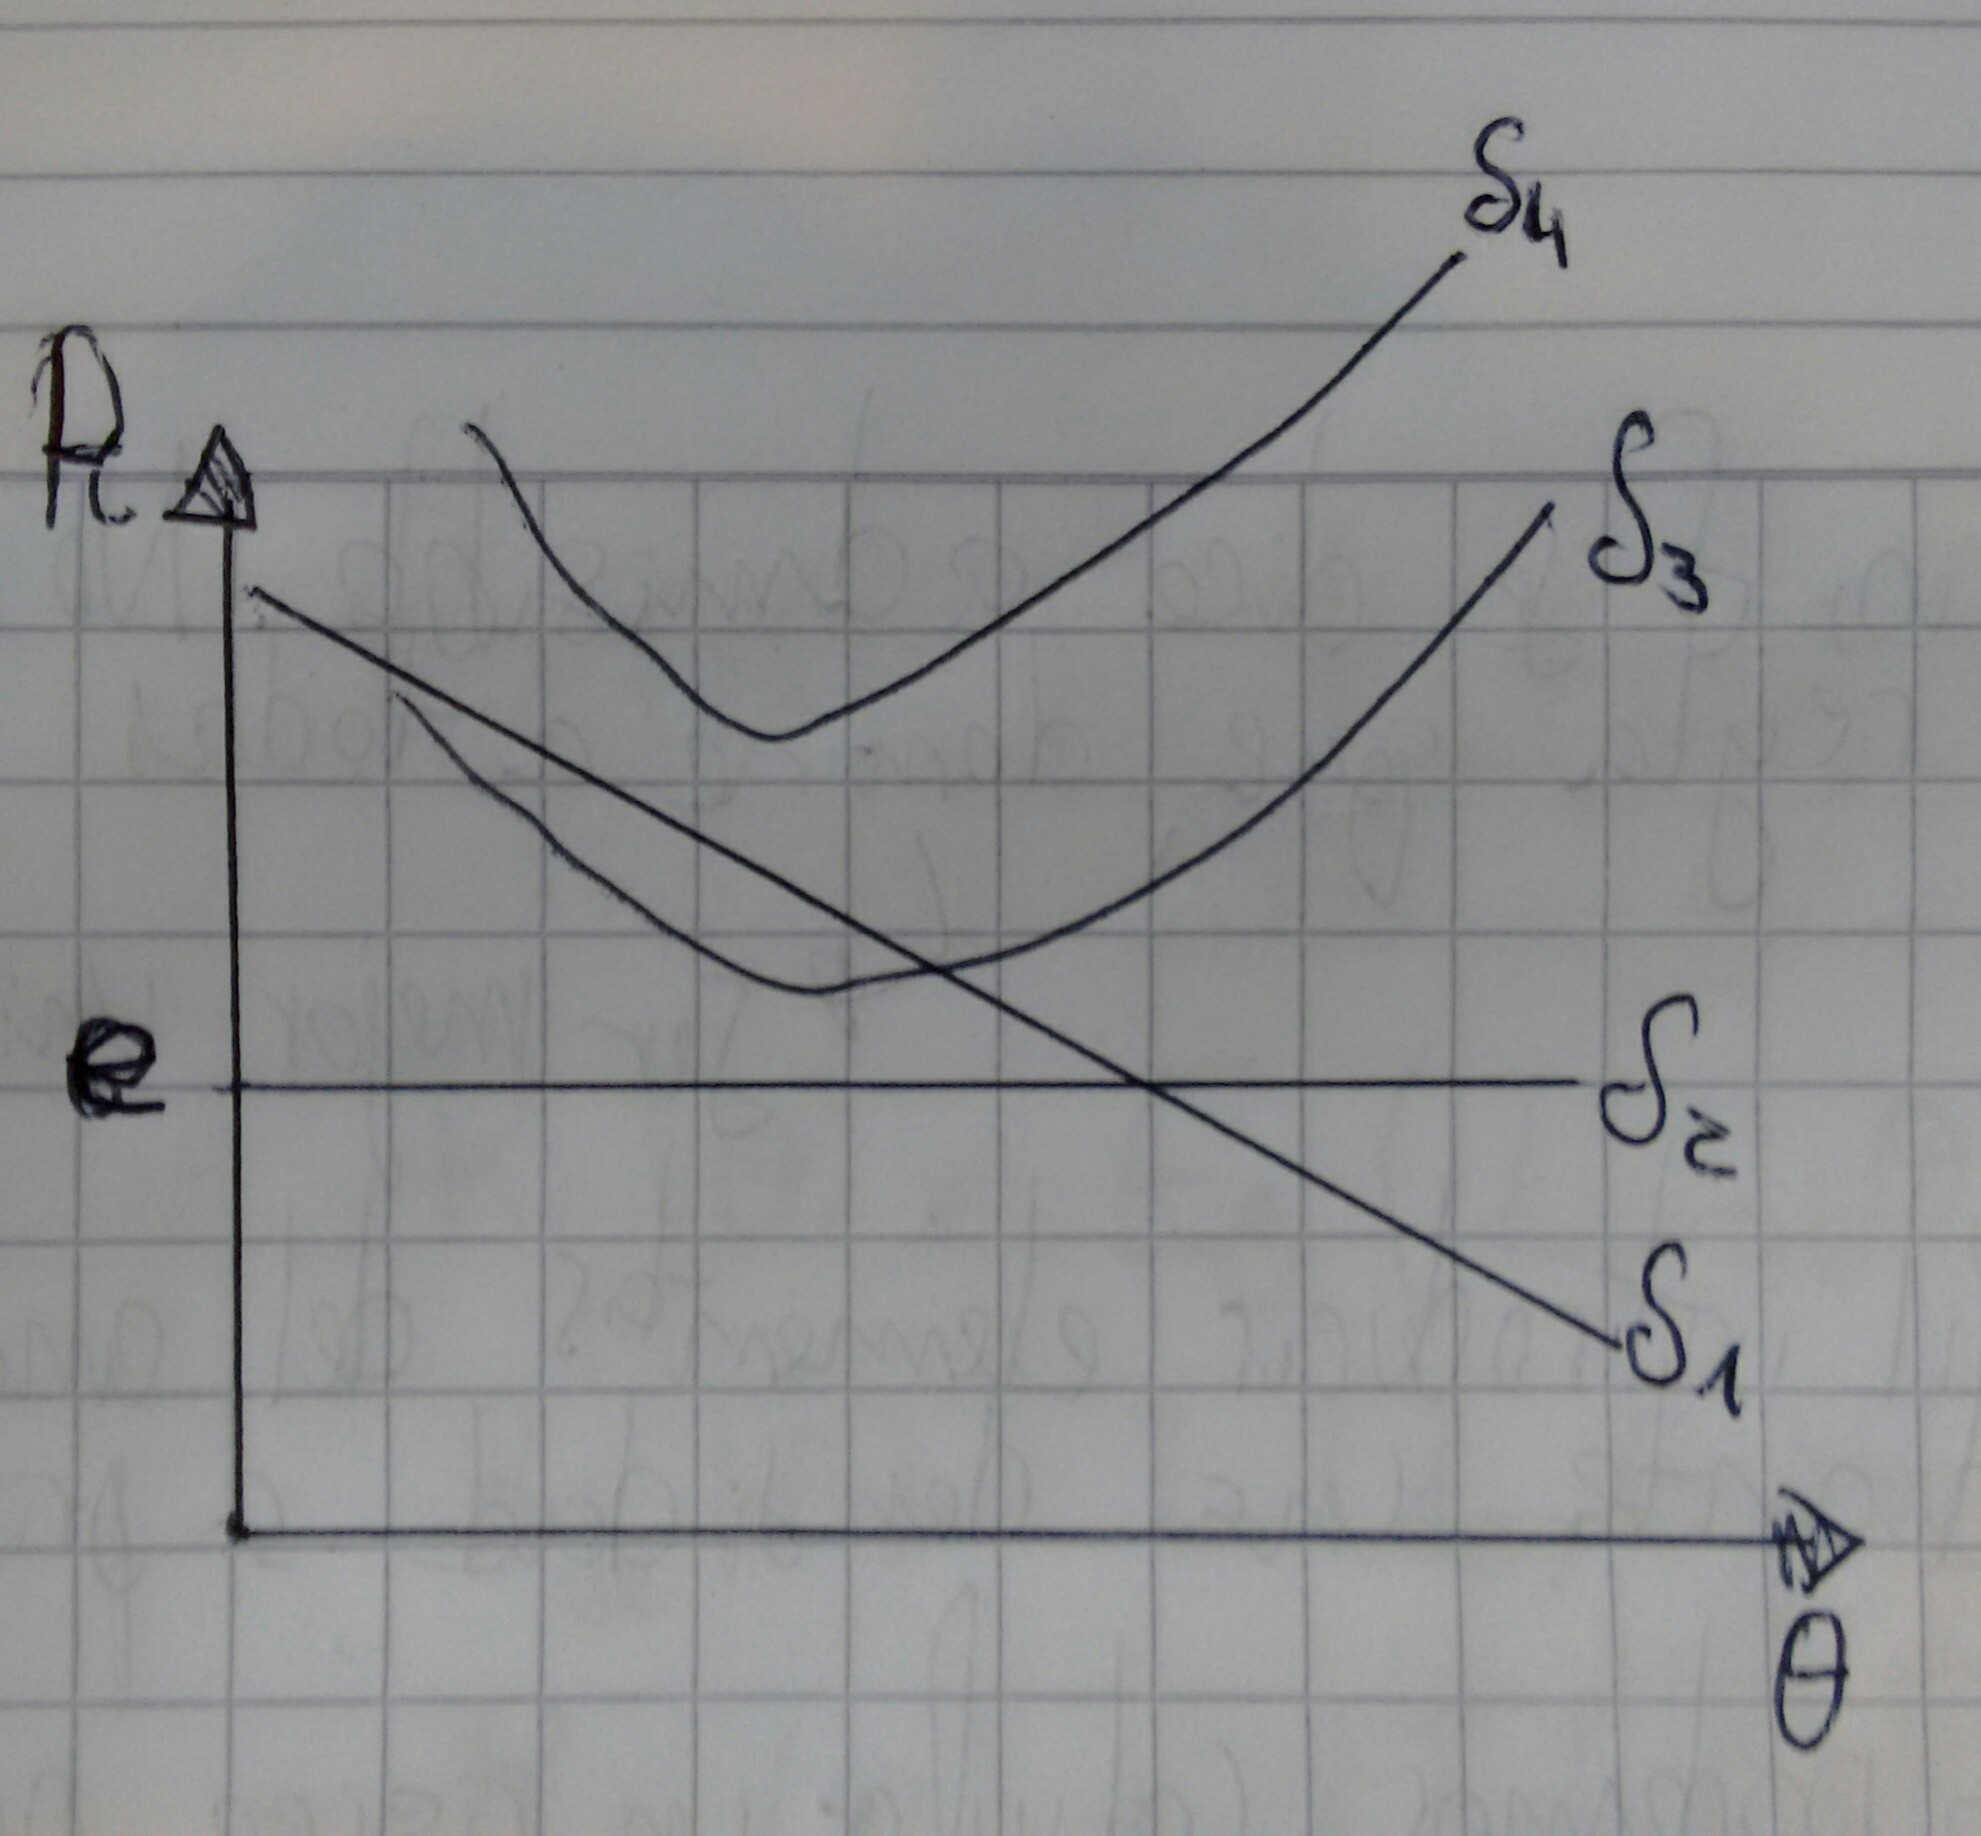
\includegraphics[scale=0.1]{imagenes/riesgo.jpg}
\end{center}
\end{ej}
Una regla $\delta$ que tiene $R_{\delta}(\theta) \ge  R_{\hat{\delta}}(\theta) \forall \theta \in \Theta, \forall \hat{\delta}$ en alguna clase. Se dice inadmisible, estas reglas salen del problema.\\

En caso contrario $\delta$ se dice admisible. No existe en general, una regla que domine a todas (ser mejor uniformemente).\\

Aquí ouede ser útil introducir elementos del análisis bayesiano, mediante una densidad a priori $\pi (\theta)$.\\
Con este elemento podemos calcular un riesgo promedio:
\begin{align*}
\bar{R_{\delta}} = \int_{\Theta} R_{\delta}(\theta) \pi(\theta) d\theta
\end{align*}
Con esto podemos buscar $\min_{\delta} \bar{R_{\delta}}$. En ejemplo, claro que existe.\\

Esto no es lo único que podemos hacer. Existe el llamado criterio de minimax. En lugar de promediar consideramos $\max_{\theta}R_{\delta}(\theta)$ y declaramos que $\delta$ es mejor que $\delta'$ si
\begin{align*}
\max_{\theta} R_{\delta}(\theta) \le \max_{\delta} R_{\delta'}(\theta)
\end{align*}
Esto suele llevar a decisiones conservadoras.
\end{document}